
%(BEGIN_QUESTION)
% Copyright 2012, Tony R. Kuphaldt, released under the Creative Commons Attribution License (v 1.0)
% This means you may do almost anything with this work of mine, so long as you give me proper credit

Et par motordrevne kompressorer arbeider sammen for å komprimere gass i et industrielt ammoniakkanlegg.  Reguleringsstrategien er laget for å fordele lasten jevnt mellom de to kompressorene, slik at ingen av dem arbeider hardere enn den andre, samtidig som begge jobber mot et felles mål:

$$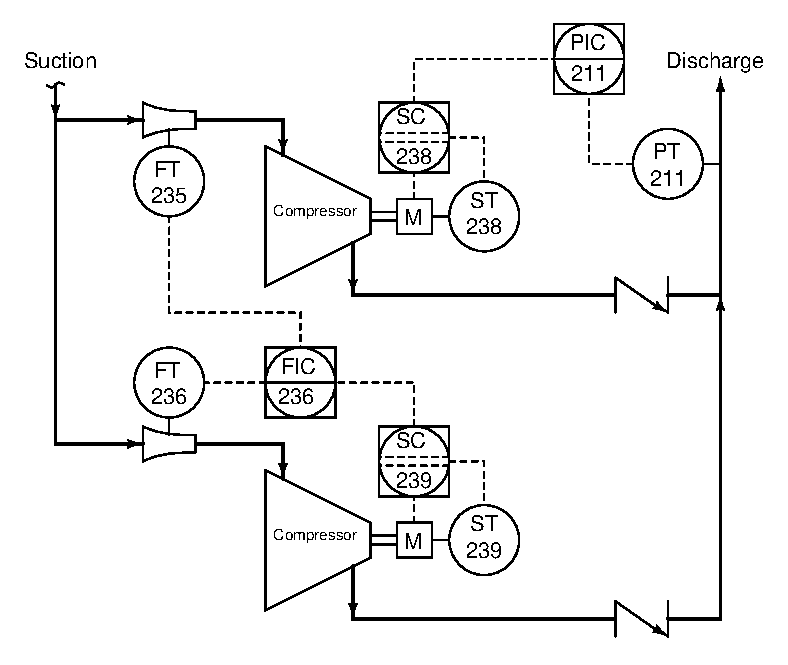
\includegraphics[width=15.5cm]{i01145x01.eps}$$

Identifiser riktig virkemåte for hver regulator i systemet, forutsatt direktevirkende transmittere og motorstyringer som øker hastigheten når 4-20 mA-signalet øker:

\vskip 10pt

FIC-236 = {\it direktevirkende} eller {\it reversvirkende}? \hskip 30pt SC-238 = {\it direktevirkende} eller {\it reversvirkende}? \hskip 30pt PIC-211 = {\it direktevirkende} eller {\it reversvirkende}?

\vskip 10pt

Anta at en operatør ber deg undersøke systemet og finne ut hvorfor utløpstrykket ikke holder settpunktet.  Ifølge operatøren fungerte alt fint i går, og har fungert fint i flere måneder.  Du går til kontrollrommet for å se DCS-visningen, og finner disse verdiene:

% No blank lines allowed between lines of an \halign structure!
% I use comments (%) instead, so that TeX doesn't choke.

$$\vbox{\offinterlineskip
\halign{\strut
\vrule \quad\hfil # \ \hfil & 
\vrule \quad\hfil # \ \hfil & 
\vrule \quad\hfil # \ \hfil \vrule \cr
\noalign{\hrule}
%
% First row
{\bf Parameter} & {\bf FIC-236} & {\bf PIC-211}  \cr
%
\noalign{\hrule}
%
% Another row
PV & 29\% & 41\%  \cr
%
\noalign{\hrule}
%
% Another row
SP & 29\% & 60\%  \cr
%
\noalign{\hrule}
%
% Another row
Output & 34\% & 100\%  \cr
%
\noalign{\hrule}
} % End of \halign 
}$$ % End of \vbox

Identifiser {\it to} ulike feil, der hver av dem alene kan forklare alle symptomer i tabellen.

\begin{itemize}
\item{} 
\vskip 50pt
\item{} 
\end{itemize}

\underbar{file i01145}
%(END_QUESTION)




%(BEGIN_ANSWER)

{\it To poeng for FIC-virkemåte, 1 poeng hver for SC-virkemåte, 1 poeng for PIC-virkemåte. 3 poeng for hver gyldige feil.}

\vskip 10pt

FIC-236 = {\bf reversvirkende} \hskip 50pt SC-238 = {\bf reversvirkende} \hskip 50pt PIC-211 = {\bf reversvirkende}

\vskip 10pt

Problemet ser ut til å være manglende evne til å oppnå høy nok gjennomstrømning selv om trykkregulatoren er mettet på 100\%.  Enhver feil som begrenser gjennomstrømningen gjennom øvre kompressor er godkjent for uttelling.  Mulige feil inkluderer:

\begin{itemize}
\item{} Skadet øvre kompressor
\item{} Skadet øvre kompressormotor
\item{} SC-238 i manuell modus (for lav utgang)
\item{} ST-238 har feilet høyt
\end{itemize}

%(END_ANSWER)





%(BEGIN_NOTES)

{\bf Denne oppgaven er kun ment for prøver/eksamen, ikke arbeidsark!}.

%(END_NOTES)
